
%%--------------------------------------------------
%% Halliday: Fundamentals of Physics
%%--------------------------------------------------


%% Chapter 05: Force and Motion--I
%%--------------------------------------------------


%% Learning Objectives
%%--------------------------------------------------

%% 5.01: Identify that a force is a vector quantity and thus has both magnitude and direction and also components.
%% 5.02: Given two or more forces acting on the same particle, add the forces as vectors to get the net force.
%% 5.03: Identify Newton's first and second laws of motion.
%% 5.04: Identify inertial reference frames.
%% 5.05: Sketch a free-body diagram for an object, showing the object as a particle and drawing the forces acting on it as vectors with their tails anchored on the particle.
%% 5.06: Apply the relationship (Newton's second law) between the net force on an object, the mass of the object, and the acceleration produced by the net force.
%% 5.07: Identify that only external forces on an object can cause the object to accelerate


%% Halliday Multiple Choice Questions
%%--------------------------------------------------
\element{halliday-mc}{
\begin{question}{halliday-ch05-q01}
    An example of an inertial reference frame is:
    \begin{choices}
        \wrongchoice{any reference frame that is not accelerating}
      \correctchoice{a frame attached to a particle on which there are no forces}
        \wrongchoice{any reference frame that is at rest}
        \wrongchoice{a reference frame attached to the center of the universe}
        \wrongchoice{a reference frame attached to Earth}
    \end{choices}
\end{question}
}

\element{halliday-mc}{
\begin{question}{halliday-ch05-q02}
    An object moving at constant velocity in an inertial frame must:
    \begin{choices}
        \wrongchoice{have a net force on it}
        \wrongchoice{eventually stop due to gravity}
        \wrongchoice{not have any force of gravity on it}
      \correctchoice{have zero net force on it}
        \wrongchoice{have no frictional force on it}
    \end{choices}
\end{question}
}

\element{halliday-mc}{
\begin{question}{halliday-ch05-q03}
    In SI units a force is numerically equal to the \rule[-0.1pt]{4em}{0.1pt}  when the force is applied to it.
    \begin{choices}
        \wrongchoice{velocity of the standard kilogram}
        \wrongchoice{speed of the standard kilogram}
        \wrongchoice{velocity of any object}
      \correctchoice{acceleration of the standard kilogram}
        \wrongchoice{acceleration of any object}
    \end{choices}
\end{question}
}

\element{halliday-mc}{
\begin{question}{halliday-ch05-q04}
    Which of the following quantities is \emph{not} a vector?
    \begin{multicols}{2}
    \begin{choices}
      \correctchoice{Mass}
        \wrongchoice{Displacement}
        \wrongchoice{Weight}
        \wrongchoice{Acceleration}
        \wrongchoice{Force}
    \end{choices}
    \end{multicols}
\end{question}
}

\element{halliday-mc}{
\begin{question}{halliday-ch05-q05}
    A newton is the force:
    \begin{choices}
        \wrongchoice{of gravity on a \SI{1}{\kilo\gram} body}
        \wrongchoice{of gravity on a \SI{1}{\gram} body}
        \wrongchoice{that gives a \SI{1}{\gram} body an acceleration of \SI{1}{\centi\meter\per\second\squared}}
      \correctchoice{that gives a \SI{1}{\kilo\gram} body an acceleration of \SI{1}{\meter\per\second\squared}}
        \wrongchoice{that gives a \SI{1}{\kilo\gram} body an acceleration of \SI{9.8}{\meter\per\second\squared}}
    \end{choices}
\end{question}
}

\element{halliday-mc}{
\begin{question}{halliday-ch05-q06}
    The unit of force called the newton is:
    \begin{multicols}{2}
    \begin{choices}
        \wrongchoice{\SI{9.8}{\kilo\gram\meter\per\second}}
      \correctchoice{\SI{1}{\kilo\gram\meter\per\second\squared}}
        \wrongchoice{defined by means of Newton's third law}
        \wrongchoice{\SI{1}{\kilo\gram} of mass}
        \wrongchoice{\SI{1}{\kilo\gram} of force}
    \end{choices}
    \end{multicols}
\end{question}
}

\element{halliday-mc}{
\begin{question}{halliday-ch05-q07}
    A force of \SI{1}{\newton} is:
    \begin{multicols}{3}
    \begin{choices}
        \wrongchoice{\SI{1}{\kilo\gram\per\second}}
        \wrongchoice{\SI{1}{\kilo\gram\meter\per\second}}
      \correctchoice{\SI{1}{\kilo\gram\meter\per\second\squared}}
        \wrongchoice{\SI{1}{\kilo\gram\meter\squared\per\second}}
        \wrongchoice{\SI{1}{\kilo\gram\meter\squared\per\second\squared}}
    \end{choices}
    \end{multicols}
\end{question}
}

\element{halliday-mc}{
\begin{question}{halliday-ch05-q08}
    The standard \SI{1}{\kilo\gram} mass is attached to a compressed spring and the spring is released.
    If the mass initially has an acceleration of \SI{5.6}{\meter\per\second\squared},
        the force of the spring has a magnitude of:
    \begin{multicols}{2}
    \begin{choices}
        \wrongchoice{\SI{2.8}{\newton}}
      \correctchoice{\SI{5.6}{\newton}}
        \wrongchoice{\SI{11.2}{\newton}}
        \wrongchoice{zero}
        \wrongchoice{an undetermined amount}
    \end{choices}
    \end{multicols}
\end{question}
}

\element{halliday-mc}{
\begin{question}{halliday-ch05-q09}
    Acceleration is always in the direction:
    \begin{choices}
        \wrongchoice{of the displacement}
        \wrongchoice{of the initial velocity}
        \wrongchoice{of the final velocity}
      \correctchoice{of the net force}
        \wrongchoice{opposite to the frictional force}
    \end{choices}
\end{question}
}

\element{halliday-mc}{
\begin{question}{halliday-ch05-q10}
    The term ``mass'' refers to the same physical concept as:
    \begin{multicols}{2}
    \begin{choices}
        \wrongchoice{weight}
      \correctchoice{inertia}
        \wrongchoice{force}
        \wrongchoice{acceleration}
        \wrongchoice{volume}
    \end{choices}
    \end{multicols}
\end{question}
}

\element{halliday-mc}{
\begin{question}{halliday-ch05-q11}
    The inertia of a body tends to cause the body to:
    \begin{choices}
        \wrongchoice{speed up}
        \wrongchoice{slow down}
      \correctchoice{resist any change in its motion}
        \wrongchoice{fall toward Earth}
        \wrongchoice{decelerate due to friction}
    \end{choices}
\end{question}
}

\element{halliday-mc}{
\begin{question}{halliday-ch05-q12}
    A heavy ball is suspended as shown.
    \begin{center}
    \begin{tikzpicture}
        \node[anchor=south,fill,pattern=north east lines,minimum width=4cm, minimum height=0.05cm] at (0,0) {};
        \draw (-2,0) -- (2,0);
        \node[draw,fill=white!90!black,circle,minimum size=1cm] (M) at (0,-2) {};
        \draw (0,0) -- (M.north) node[pos=0.5,anchor=west] {upper string};
        \draw (M.south) -- ++(270:1.5) node[pos=0.5,anchor=west] {lower string};
    \end{tikzpicture}
    \end{center}
    A quick jerk on the lower string will break that string but a slow pull on the lower string will break the upper string.
    The first result occurs because:
    \begin{choices}
        \wrongchoice{the force is too small to move the ball}
        \wrongchoice{action and reaction is operating}
      \correctchoice{the ball has inertia}
        \wrongchoice{air friction holds the ball back}
        \wrongchoice{the ball has too much energy}
    \end{choices}
\end{question}
}

\element{halliday-mc}{
\begin{question}{halliday-ch05-q13}
    When a certain force is applied to the standard kilogram its acceleration is \SI{5.0}{\meter\per\second\squared}.
    When the same force is applied to another object its acceleration is one-fifth as much.
    The mass of the object is:
    \begin{multicols}{3}
    \begin{choices}
        \wrongchoice{\SI{0.2}{\kilo\gram}}
        \wrongchoice{\SI{0.5}{\kilo\gram}}
        \wrongchoice{\SI{1.0}{\kilo\gram}}
      \correctchoice{\SI{5.0}{\kilo\gram}}
        \wrongchoice{\SI{10}{\kilo\gram}}
    \end{choices}
    \end{multicols}
\end{question}
}

\element{halliday-mc}{
\begin{question}{halliday-ch05-q14}
    Mass differs from weight in that:
    \begin{choices}
        \wrongchoice{all objects have weight but some lack mass}
      \correctchoice{weight is a force and mass is not}
        \wrongchoice{the mass of an object is always more than its weight}
        \wrongchoice{mass can be expressed only in the metric system}
        \wrongchoice{there is no difference}
    \end{choices}
\end{question}
}

\element{halliday-mc}{
\begin{question}{halliday-ch05-q15}
    The mass of a body:
    \begin{choices}
        \wrongchoice{is slightly different at different places on Earth}
        \wrongchoice{is a vector}
      \correctchoice{is independent of the free-fall acceleration}
        \wrongchoice{is the same for all bodies of the same volume}
        \wrongchoice{can be measured most accurately on a spring scale}
    \end{choices}
\end{question}
}

\element{halliday-mc}{
\begin{question}{halliday-ch05-q16}
    The mass and weight of a body:
    \begin{choices}
        \wrongchoice{differ by a factor of 9.8}
        \wrongchoice{are identical}
        \wrongchoice{are the same physical quantities expressed in different units}
        \wrongchoice{are both a direct measure of the inertia of the body}
      \correctchoice{have the same ratio as that of any other body placed at that location}
    \end{choices}
\end{question}
}

\element{halliday-mc}{
\begin{question}{halliday-ch05-q17}
    An object placed on an equal-arm balance requires \SI{12}{\kilo\gram} to balance it.
    When placed on a spring scale, the scale reads \SI{12}{\kilo\gram}.
    Everything (balance, scale, set of weights and object) is now transported to the Moon where the free-fall acceleration is one-sixth that on Earth.
    The new readings of the balance and spring scale (respectively) are:
    \begin{multicols}{2}
    \begin{choices}
        \wrongchoice{\SI{12}{\kilo\gram}, \SI{12}{\kilo\gram}}
        \wrongchoice{\SI{2}{\kilo\gram}, \SI{2}{\kilo\gram}}
      \correctchoice{\SI{12}{\kilo\gram}, \SI{2}{\kilo\gram}}
        \wrongchoice{\SI{2}{\kilo\gram}, \SI{12}{\kilo\gram}}
        \wrongchoice{\SI{12}{\kilo\gram}, \SI{72}{\kilo\gram}}
    \end{choices}
    \end{multicols}
\end{question}
}

\element{halliday-mc}{
\begin{question}{halliday-ch05-q18}
    Two objects, one having three times the mass of the other,
        are dropped from the same height in a vacuum.
    At the end of their fall, their velocities are equal because:
    \begin{choices}
        \wrongchoice{anything falling in vacuum has constant velocity}
        \wrongchoice{all objects reach the same terminal velocity}
        \wrongchoice{the acceleration of the larger object is three times greater than that of the smaller object}
        \wrongchoice{the force of gravity is the same for both objects}
      \correctchoice{none of the provided}
    \end{choices}
\end{question}
}

\element{halliday-mc}{
\begin{question}{halliday-ch05-q19}
    A feather and a lead ball are dropped from rest in vacuum on the Moon.
    The acceleration of the feather is:
    \begin{choices}
        \wrongchoice{more than that of the lead ball}
      \correctchoice{the same as that of the lead ball}
        \wrongchoice{less than that of the lead ball}
        \wrongchoice{\SI{9.8}{\meter\per\second\squared}}
        \wrongchoice{zero since it floats in a vacuum}
    \end{choices}
\end{question}
}

\element{halliday-mc}{
\begin{question}{halliday-ch05-q20}
    The block shown moves with constant velocity on a horizontal surface.
    Two of the forces on it are shown.
    \begin{center}
    \begin{tikzpicture}
        %% Ground
        \node[anchor=north,fill,pattern=north east lines,minimum width=4cm,minimum height=0.05cm] at (0,0) {};
        \draw (-2,0) -- (2,0);
        %% Mass
        \node[draw,fill=white!90!black,minimum size=1.22cm,anchor=south] (M) at (0,0) {};
        %% Vectors
        \draw[thick,->] (M.east) -- ++(0:1.5cm) node[anchor=south,pos=0.5] {\SI{5}{\newton}};
        \draw[thick,->] (M.west) -- ++(180:0.9cm) node[anchor=south,pos=0.5] {\SI{3}{\newton}};
    \end{tikzpicture}
    \end{center}
    A frictional force exerted by the surface is the only other horizontal force on the block.
    The frictional force is:
    \begin{choices}
        \wrongchoice{zero}
      \correctchoice{\SI{2}{\newton}, leftward}
        \wrongchoice{\SI{2}{\newton}, rightward}
        \wrongchoice{slightly more than \SI{2}{\newton}, leftward}
        \wrongchoice{slightly less than \SI{2}{\newton}, leftward}
    \end{choices}
\end{question}
}

\element{halliday-mc}{
\begin{question}{halliday-ch05-q21}
    Two forces, one with a magnitude of \SI{3}{\newton} and the other with a magnitude of \SI{5}{\newton},
        are applied to an object.
    For which orientations of the forces shown in the diagrams is the magnitude of the acceleration of the object the least?
    \begin{multicols}{2}
    \begin{choices}
        %% ANS: is A
        \AMCboxDimensions{down=-0.8cm}
        \correctchoice{
            \begin{tikzpicture}
                \draw[white] (-1,-1) rectangle (1.5,1);
                \node[draw,fill=white!90!black,minimum size=0.25cm,anchor=center] (M) at (0,0) {};
                \draw[thick,->] (M.east) -- ++(0:1.5) node[anchor=south,pos=0.8] {\SI{5}{\newton}};
                \draw[thick,->] (M.west) -- ++(180:0.9) node[anchor=south,pos=0.8] {\SI{3}{\newton}};
            \end{tikzpicture}
        }
        \wrongchoice{
            \begin{tikzpicture}
                \draw[white] (-1,-1) rectangle (1.5,1);
                \node[draw,fill=white!90!black,minimum size=0.25cm,anchor=center] (M) at (0,0) {};
                \draw[thick,->] (M.east) -- ++(0:1.5) node[anchor=south,pos=0.8] {\SI{5}{\newton}};
                \draw[thick,->] (M.north) -- ++(90:0.9) node[anchor=west,pos=0.8] {\SI{3}{\newton}};
            \end{tikzpicture}
        }
        \wrongchoice{
            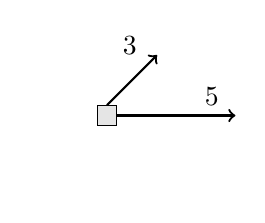
\begin{tikzpicture}
                \draw[white] (-1,-1) rectangle (1.5,1);
                \node[draw,fill=white!90!black,minimum size=0.25cm,anchor=center] (M) at (0,0) {};
                \draw[thick,->] (M.east) -- ++(0:1.5) node[anchor=south,pos=0.8] {\SI{5}{\newton}};
                \draw[thick,->] (M.north) -- ++(45:0.9) node[anchor=south east,pos=0.8] {\SI{3}{\newton}};
            \end{tikzpicture}
        }
        \wrongchoice{
            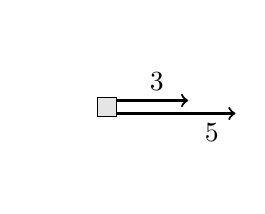
\begin{tikzpicture}
                \draw[white] (-1,-1) rectangle (1.5,1);
                \node[draw,fill=white!90!black,minimum size=0.25cm,anchor=center] (M) at (0,0) {};
                \draw[thick,->] (M.south east) ++(90:0.05) -- ++(0:1.5) node[anchor=north,pos=0.8] {\SI{5}{\newton}};
                \draw[thick,->] (M.north east) ++(270:0.05) -- ++(0:0.9) node[anchor=south east,pos=0.8] {\SI{3}{\newton}};
            \end{tikzpicture}
        }
        \wrongchoice{
            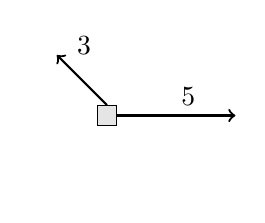
\begin{tikzpicture}
                \draw[white] (-1,-1) rectangle (1.5,1);
                \node[draw,fill=white!90!black,minimum size=0.25cm,anchor=center] (M) at (0,0) {};
                \draw[thick,->] (M.east) -- ++(0:1.5) node[anchor=south,pos=0.6] {\SI{5}{\newton}};
                \draw[thick,->] (M.north) -- ++(135:0.9) node[anchor=south west,pos=0.8] {\SI{3}{\newton}};
            \end{tikzpicture}
        }
    \end{choices}
    \end{multicols}
\end{question}
}

\element{halliday-mc}{
\begin{question}{halliday-ch05-q22}
    A crate rests on a horizontal surface and a woman pulls on it with a \SI{10}{\newton} force.
    Rank the situations shown below according to the magnitude of the normal force exerted by the surface on the crate,
        least to greatest.
    \begin{center}
    \begin{tikzpicture}
        %% Ground
        \node[anchor=north,fill,pattern=north east lines,minimum width=2cm, minimum height=0.05cm] at (0,0) {};
        \draw (-1,0) -- (1,0);
        \node[anchor=north,yshift=-0.20cm] at (0,0) {$1$};
        %% Mass
        \node[draw,fill=white!90!black,minimum size=0.75cm,anchor=south] (M) at (0,0) {};
        %% Vectors
        \draw[thick,->] (M.east) -- ++(0:1.5cm) node[anchor=south,pos=0.5] {\SI{10}{\newton}};
    \end{tikzpicture}
    \begin{tikzpicture}
        %% Ground
        \node[anchor=north,fill,pattern=north east lines,minimum width=2cm, minimum height=0.05cm] at (0,0) {};
        \draw (-1,0) -- (1,0);
        \node[anchor=north,yshift=-0.20cm] at (0,0) {$2$};
        %% Mass
        \node[draw,fill=white!90!black,minimum size=0.75cm,anchor=south] (M) at (0,0) {};
        %% Vectors
        \draw[thick,->] (M.east) -- ++(45:1.5cm) node[anchor=south east,pos=0.8] {\SI{10}{\newton}};
    \end{tikzpicture}
    \begin{tikzpicture}
        %% Ground
        \node[anchor=north,fill,pattern=north east lines,minimum width=2cm, minimum height=0.05cm] at (0,0) {};
        \draw (-1,0) -- (1,0);
        \node[anchor=north,yshift=-0.20cm] at (0,0) {$3$};
        %% Mass
        \node[draw,fill=white!90!black,minimum size=0.75cm,anchor=south] (M) at (0,0) {};
        %% Vectors
        \draw[thick,->] (M.north) -- ++(90:1.5cm) node[anchor=west,pos=0.5] {\SI{10}{\newton}};
    \end{tikzpicture}
    \end{center}
    \begin{multicols}{2}
    \begin{choices}
        %% ANS: is E
        \wrongchoice{1, 2, 3}
        \wrongchoice{2, 1, 3}
        \wrongchoice{2, 3, 1}
        \wrongchoice{1, 3, 2}
      \correctchoice{3, 2, 1}
    \end{choices}
    \end{multicols}
\end{question}
}

\element{halliday-mc}{
\begin{question}{halliday-ch05-q23}
    A heavy wooden block is dragged by a force $F$ along a rough steel plate,
        as shown in the diagrams for two cases.
    \begin{center}
    \begin{tikzpicture}
        %% Ground
        \node[anchor=north,fill,pattern=north east lines,minimum width=2cm, minimum height=0.05cm] at (0,0) {};
        \draw (-1,0) -- (1,0);
        \node[anchor=north,yshift=-0.15cm] at (0,0) {(i)};
        %% Mass
        \node[draw,fill=white!90!black,minimum size=1cm,anchor=south] (M) at (0,0) {};
        %% Vectors
        \draw[thick,->] (M.east) -- ++(0:1.5cm) node[anchor=south,pos=0.5] {$\vec{F}$};
    \end{tikzpicture}
    \begin{tikzpicture}
        %% Ground
        \node[anchor=north,fill,pattern=horizontal lines,minimum width=2cm, minimum height=0.05cm,rotate=45] at (0,0) {};
        \draw (225:1) -- (45:1);
        \node[anchor=north west,yshift=-0.08cm,xshift=0.08cm] at (0,0) {(ii)};
        %% Mass
        \node[draw,fill=white!90!black,minimum size=1cm,anchor=south,rotate=45] (M) at (0,0) {};
        %% Vectors
        \draw[thick,->] (M.east) -- ++(45:1.5cm) node[anchor=south,pos=0.5] {$\vec{F}$};
    \end{tikzpicture}
    \end{center}
    The magnitude of the applied force $F$ is the same for both cases.
    The normal force in (ii),
        as compared with the normal force in (i) is:
    \begin{choices}
        \wrongchoice{the same}
        \wrongchoice{greater}
      \correctchoice{less}
        \wrongchoice{less for some angles of the incline and greater for others}
        \wrongchoice{less or greater, depending on the magnitude of the applied force $F$.}
    \end{choices}
\end{question}
}

\element{halliday-mc}{
\begin{question}{halliday-ch05-q24}
    Equal forces $F$ act on isolated bodies $A$ and $B$.
    The mass of $B$ is three times that of $A$.
    The magnitude of the acceleration of $A$ is:
    \begin{choices}
      \correctchoice{three times that of $B$}
        \wrongchoice{1/3 that of $B$}
        \wrongchoice{the same as $B$}
        \wrongchoice{nine times that of $B$}
        \wrongchoice{1/9 that of $B$}
    \end{choices}
\end{question}
}

\element{halliday-mc}{
\begin{question}{halliday-ch05-q25}
    A car travels east at constant velocity.
    The net force on the car is:
    \begin{multicols}{3}
    \begin{choices}
        \wrongchoice{east}
        \wrongchoice{west}
        \wrongchoice{up}
        \wrongchoice{down}
      \correctchoice{zero}
    \end{choices}
    \end{multicols}
\end{question}
}

\element{halliday-mc}{
\begin{question}{halliday-ch05-q26}
    A constant force of \SI{8.0}{\newton} is exerted for \SI{4.0}{\second} on a \SI{16}{\kilo\gram} object initially at rest.
    The change in speed of this object will be:
    \begin{multicols}{3}
    \begin{choices}
        \wrongchoice{\SI{0.5}{\meter\per\second}}
      \correctchoice{\SI{2}{\meter\per\second}}
        \wrongchoice{\SI{4}{\meter\per\second}}
        \wrongchoice{\SI{8}{\meter\per\second}}
        \wrongchoice{\SI{32}{\meter\per\second}}
    \end{choices}
    \end{multicols}
\end{question}
}

\element{halliday-mc}{
\begin{question}{halliday-ch05-q27}
    A \SI{6}{\kilo\gram} object is moving south.
    A net force of \SI{12}{\newton} north on it results in the object having an acceleration of:
    \begin{multicols}{2}
    \begin{choices}
      \correctchoice{\SI{2}{\meter\per\second\squared}, north}
        \wrongchoice{\SI{2}{\meter\per\second\squared}, south}
        \wrongchoice{\SI{6}{\meter\per\second\squared}, north}
        \wrongchoice{\SI{18}{\meter\per\second\squared}, north}
        \wrongchoice{\SI{18}{\meter\per\second\squared}, south}
    \end{choices}
    \end{multicols}
\end{question}
}

\element{halliday-mc}{
\begin{question}{halliday-ch05-q28}
    A \SI{9000}{\newton} automobile is pushed along a level road by four students who apply a total forward force of \SI{500}{\newton}.
    Neglecting friction, the acceleration of the automobile is:
    \begin{multicols}{2}
    \begin{choices}
        \wrongchoice{\SI{0.055}{\meter\per\second\squared}}
      \correctchoice{\SI{0.54}{\meter\per\second\squared}}
        \wrongchoice{\SI{1.8}{\meter\per\second\squared}}
        \wrongchoice{\SI{9.8}{\meter\per\second\squared}}
        \wrongchoice{\SI{18}{\meter\per\second\squared}}
    \end{choices}
    \end{multicols}
\end{question}
}

\element{halliday-mc}{
\begin{question}{halliday-ch05-q29}
    An object rests on a horizontal frictionless surface.
    A horizontal force of magnitude $F$ is applied.
    This force produces an acceleration:
    \begin{choices}
        \wrongchoice{only if $F$ is larger than the weight of the object}
        \wrongchoice{only while the object suddenly changes from rest to motion}
      \correctchoice{always}
        \wrongchoice{only if the inertia of the object decreases}
        \wrongchoice{only if $F$ is increasing}
    \end{choices}
\end{question}
}

\element{halliday-mc}{
\begin{question}{halliday-ch05-q30}
    A \SI{25}{\kilo\gram} crate is pushed across a frictionless horizontal floor with a force of \SI{20}{\newton},
        directed \ang{20} below the horizontal.
    The acceleration of the crate is:
    \begin{multicols}{2}
    \begin{choices}
        \wrongchoice{\SI{0.27}{\meter\per\second\squared}}
      \correctchoice{\SI{0.75}{\meter\per\second\squared}}
        \wrongchoice{\SI{0.80}{\meter\per\second\squared}}
        \wrongchoice{\SI{170}{\meter\per\second\squared}}
        \wrongchoice{\SI{470}{\meter\per\second\squared}}
    \end{choices}
    \end{multicols}
\end{question}
}

\element{halliday-mc}{
\begin{question}{halliday-ch05-q31}
    A ball with a weight of \SI{1.5}{\newton} is thrown at an angle of \ang{30} above the horizontal with an initial speed of \SI{12}{\meter\per\second}.
    At its highest point,
        the net force on the ball is:
    \begin{choices}
        \wrongchoice{\SI{9.8}{\newton}, \ang{30} below horizontal}
        \wrongchoice{zero}
        \wrongchoice{\SI{9.8}{\newton}, up}
        \wrongchoice{\SI{9.8}{\newton}, down}
      \correctchoice{\SI{1.5}{\newton}, down}
    \end{choices}
\end{question}
}

\element{halliday-mc}{
\begin{question}{halliday-ch05-q32}
    Two forces are applied to a \SI{5.0}{\kilo\gram} crate;
        one is \SI{6.0}{\newton} to the north and the other is \SI{8.0}{\newton} to the west.
    The magnitude of the acceleration of the crate is:
    \begin{multicols}{3}
    \begin{choices}
        \wrongchoice{\SI{0.50}{\meter\per\second\squared}}
      \correctchoice{\SI{2.0}{\meter\per\second\squared}}
        \wrongchoice{\SI{2.8}{\meter\per\second\squared}}
        \wrongchoice{\SI{10}{\meter\per\second\squared}}
        \wrongchoice{\SI{50}{\meter\per\second\squared}}
    \end{choices}
    \end{multicols}
\end{question}
}

\element{halliday-mc}{
\begin{question}{halliday-ch05-q33}
    A \SI{400}{\newton} steel ball is suspended by a light rope from the ceiling.
    The tension in the rope is:
    \begin{multicols}{3}
    \begin{choices}
      \correctchoice{\SI{400}{\newton}}
        \wrongchoice{\SI{800}{\newton}}
        \wrongchoice{zero}
        \wrongchoice{\SI{200}{\newton}}
        \wrongchoice{\SI{560}{\newton}}
    \end{choices}
    \end{multicols}
\end{question}
}

\element{halliday-mc}{
\begin{question}{halliday-ch05-q34}
    A heavy steel ball $B$ is suspended by a cord from a block of wood $W$.
    The entire system is dropped through the air.
    Neglecting air resistance, the tension in the cord is:
    \begin{choices}
      \correctchoice{zero}
        \wrongchoice{the difference in the masses of $B$ and $W$}
        \wrongchoice{the difference in the weights of $B$ and $W$}
        \wrongchoice{the weight of $B$}
        \wrongchoice{none of these}
    \end{choices}
\end{question}
}

%\element{halliday-mc}{
%\begin{question}{halliday-ch05-q35}
%    A circus performer of weight W is walking along a ``high wire'' as shown.
%    \begin{center}
%        %% NOTE:
%    \end{center}
%    The tension in the wire:
%    \begin{choices}
%        \wrongchoice{is approximately $W$}
%        \wrongchoice{is approximately $W/2$}
%        \wrongchoice{is much less than $W$}
%      \correctchoice{is much more than $W$}
%        \wrongchoice{depends on whether he stands on one foot or two feet}
%    \end{choices}
%\end{question}
%}

\element{halliday-mc}{
\begin{question}{halliday-ch05-q36}
    A \SI{1000}{\kilo\gram} elevator is rising and its speed is increasing at \SI{3 }{\meter\per\second\squared}.
    The tension force of the cable on the elevator is:
    \begin{multicols}{2}
    \begin{choices}
        \wrongchoice{\SI{6800}{\newton}}
        \wrongchoice{\SI{1000}{\newton}}
        \wrongchoice{\SI{3000}{\newton}}
        \wrongchoice{\SI{9800}{\newton}}
      \correctchoice{\SI{12800}{\newton}}
    \end{choices}
    \end{multicols}
\end{question}
}

\element{halliday-mc}{
\begin{question}{halliday-ch05-q37}
    A \SI{5}{\kilo\gram} block is suspended by a rope from the ceiling of an elevator as the elevator accelerates downward at \SI{3.0}{\meter\per\second}.
    The tension force of the rope on the block is:
    \begin{multicols}{2}
    \begin{choices}
        \wrongchoice{\SI{15}{\newton}, up}
      \correctchoice{\SI{34}{\newton}, up}
        \wrongchoice{\SI{34}{\newton}, down}
        \wrongchoice{\SI{64}{\newton}, up}
        \wrongchoice{\SI{64}{\newton}, down}
    \end{choices}
    \end{multicols}
\end{question}
}

\element{halliday-mc}{
\begin{question}{halliday-ch05-q38}
    A crane operator lowers a \SI{16 000}{\newton} steel ball with a downward acceleration of \SI{3}{\meter\per\second\squared}.
    The tension force of the cable is:
    \begin{multicols}{2}
    \begin{choices}
        \wrongchoice{\SI{4900}{\newton}}
      \correctchoice{\SI{11 000}{\newton}}
        \wrongchoice{\SI{16 000}{\newton}}
        \wrongchoice{\SI{21 000}{\newton}}
        \wrongchoice{\SI{48 000}{\newton}}
    \end{choices}
    \end{multicols}
\end{question}
}

\element{halliday-mc}{
\begin{question}{halliday-ch05-q39}
    A \SI{1}{\newton} pendulum bob is held at an angle $\theta$ from the vertical by a \SI{2}{\newton} horizontal force $F$ as shown.
    \begin{center}
    \begin{tikzpicture}
        \node[anchor=south,fill,pattern=north east lines,minimum width=2cm, minimum height=0.05cm] at (0,0) {};
        \draw (-1,0) -- (1,0);
        \node[draw,fill=white!90!black,circle,minimum size=0.25cm] (M) at (300:3) {};
        \draw[dashed] (0,0) -- (270:2.5);
        \draw[thick] (0,0) -- (300:2.80);
        \draw[dashed] (270:1.5) arc(270:300:1.5) node[pos=0.5,anchor=north] {$\theta$};
        \draw[thick,->] (M.east) -- ++(0:1.5)  node[pos=0.5,anchor=south] {$\vec{F}$};
    \end{tikzpicture}
    \end{center}
    %The tension in the string supporting the pendulum bob (in newtons) is:
    The tension in the string supporting the pendulum bob is:
    \begin{multicols}{2}
    \begin{choices}
        \wrongchoice{$\left(\cos\theta\right)\,\si{\newton}$}
        \wrongchoice{$\left(\dfrac{2}{\cos\theta}\right)\,\si{\newton}$}
      \correctchoice{$\sqrt{5}\,\si{\newton}$}
        \wrongchoice{\SI{1}{\newton}}
        %\wrongchoice{$\cos\theta$}
        %\wrongchoice{$\dfrac{2}{\cos\theta}$}
        %\correctchoice{$\sqrt{5}$}
        %\wrongchoice{$1$}
        \wrongchoice{none of the provided}
    \end{choices}
    \end{multicols}
\end{question}
}

\element{halliday-mc}{
\begin{question}{halliday-ch05-q40}
    A car moves horizontally with a constant acceleration of \SI{3}{\meter\per\second\squared}.
    A ball is suspended by a string from the ceiling of the car. 
    The ball does not swing, being at rest with respect to the car.
    What angle does the string make with the vertical?
    \begin{choices}
      \correctchoice{\ang{17}}
        \wrongchoice{\ang{35}}
        \wrongchoice{\ang{52}}
        \wrongchoice{\ang{73}}
        \wrongchoice{Cannot be found without knowing the length of the string}
    \end{choices}
\end{question}
}

\element{halliday-mc}{
\begin{question}{halliday-ch05-q41}
    A man weighing \SI{700}{\newton} is in an elevator that is accelerating upward at \SI{4}{\meter\per\second}.
    The force exerted on him by the elevator floor is:
    \begin{multicols}{3}
    \begin{choices}
        \wrongchoice{\SI{71}{\newton}}
        \wrongchoice{\SI{290}{\newton}}
        \wrongchoice{\SI{410}{\newton}}
        \wrongchoice{\SI{700}{\newton}}
      \correctchoice{\SI{990}{\newton}}
    \end{choices}
    \end{multicols}
\end{question}
}

\element{halliday-mc}{
\begin{question}{halliday-ch05-q42}
    You stand on a spring scale on the floor of an elevator.
    Of the following,
        the scale shows the highest reading when the elevator:
    \begin{choices}
      \correctchoice{moves upward with increasing speed}
        \wrongchoice{moves upward with decreasing speed}
        \wrongchoice{remains stationary}
        \wrongchoice{moves downward with increasing speed}
        \wrongchoice{moves downward at constant speed}
    \end{choices}
\end{question}
}

\element{halliday-mc}{
\begin{question}{halliday-ch05-q43}
    You stand on a spring scale on the floor of an elevator.
    Of the following,
        the scale shows the highest reading when the elevator:
    \begin{choices}
        \wrongchoice{moves downward with increasing speed}
      \correctchoice{moves downward with decreasing speed}
        \wrongchoice{remains stationary}
        \wrongchoice{moves upward with decreasing speed}
        \wrongchoice{moves upward at constant speed}
    \end{choices}
\end{question}
}

\element{halliday-mc}{
\begin{question}{halliday-ch05-q44}
    When a \SI{25}{\kilo\gram} crate is pushed across a frictionless horizontal floor with a force of \SI{200}{\newton}, directed \ang{20} below the horizontal,
        the magnitude of the normal force of the floor on the crate is:
    \begin{multicols}{3}
    \begin{choices}
        \wrongchoice{\SI{25}{\newton}}
        \wrongchoice{\SI{68}{\newton}}
        \wrongchoice{\SI{180}{\newton}}
        \wrongchoice{\SI{250}{\newton}}
      \correctchoice{\SI{310}{\newton}}
    \end{choices}
    \end{multicols}
\end{question}
}

\element{halliday-mc}{
\begin{question}{halliday-ch05-q45}
    A block slides down a frictionless plane that makes an angle of \ang{30} with the horizontal.
    The acceleration of the block is:
    \begin{multicols}{2}
    \begin{choices}
        \wrongchoice{\SI{980}{\centi\meter\per\second\squared}}
        \wrongchoice{\SI{566}{\centi\meter\per\second\squared}}
        \wrongchoice{\SI{849}{\centi\meter\per\second\squared}}
        \wrongchoice{zero}
      \correctchoice{\SI{490}{\centi\meter\per\second\squared}}
    \end{choices}
    \end{multicols}
\end{question}
}

\element{halliday-mc}{
\begin{question}{halliday-ch05-q46}
    A \SI{25}{\newton} crate slides down a frictionless incline that is \ang{25} above the horizontal.
    The magnitude of the normal force of the incline on the crate is:
    \begin{multicols}{3}
    \begin{choices}
        \wrongchoice{\SI{11}{\newton}}
      \correctchoice{\SI{23}{\newton}}
        \wrongchoice{\SI{25}{\newton}}
        \wrongchoice{\SI{100}{\newton}}
        \wrongchoice{\SI{220}{\newton}}
    \end{choices}
    \end{multicols}
\end{question}
}

\element{halliday-mc}{
\begin{question}{halliday-ch05-q47}
    A \SI{25}{\newton} crate is held at rest on a frictionless incline by a force that is parallel to the incline.
    If the incline is \ang{25} above the horizontal the magnitude of the applied force is:
    \begin{multicols}{3}
    \begin{choices}
        \wrongchoice{\SI{4.1}{\newton}}
        \wrongchoice{\SI{4.6}{\newton}}
        \wrongchoice{\SI{8.9}{\newton}}
      \correctchoice{\SI{11}{\newton}}
        \wrongchoice{\SI{23}{\newton}}
    \end{choices}
    \end{multicols}
\end{question}
}

\element{halliday-mc}{
\begin{question}{halliday-ch05-q48}
    A \SI{25}{\newton} crate is held at rest on a frictionless incline by a force that is parallel to the incline.
    If the incline is \ang{25} above the horizontal the magnitude of the normal force of the incline on the crate is:
    \begin{multicols}{3}
    \begin{choices}
        \wrongchoice{\SI{4.1}{\newton}}
        \wrongchoice{\SI{4.6}{\newton}}
        \wrongchoice{\SI{8.9}{\newton}}
        \wrongchoice{\SI{11}{\newton}}
      \correctchoice{\SI{23}{\newton}}
    \end{choices}
    \end{multicols}
\end{question}
}

\element{halliday-mc}{
\begin{question}{halliday-ch05-q49}
    A \SI{32}{\newton} force, parallel to the incline,
        is required to push a certain crate at constant velocity up a frictionless incline that is \ang{30} above the horizontal.
    The mass of the crate is:
    \begin{multicols}{3}
    \begin{choices}
        \wrongchoice{\SI{3.3}{\kilo\gram}}
        \wrongchoice{\SI{3.8}{\kilo\gram}}
        \wrongchoice{\SI{5.7}{\kilo\gram}}
      \correctchoice{\SI{6.5}{\kilo\gram}}
        \wrongchoice{\SI{160}{\kilo\gram}}
    \end{choices}
    \end{multicols}
\end{question}
}

\element{halliday-mc}{
\begin{question}{halliday-ch05-q50}
    A sled is on an icy (frictionless) slope that is \ang{30} above the horizontal.
    When a \SI{40}{\newton} force, parallel to the incline and directed up the incline,
        is applied to the sled, the acceleration of the sled is \SI{2.0}{\meter\per\second\squared},
        down the incline.
    The mass of the sled is:
    \begin{multicols}{3}
    \begin{choices}
        \wrongchoice{\SI{3.8}{\kilo\gram}}
        \wrongchoice{\SI{4.1}{\kilo\gram}}
        \wrongchoice{\SI{5.8}{\kilo\gram}}
        \wrongchoice{\SI{6.2}{\kilo\gram}}
      \correctchoice{\SI{10}{\kilo\gram}}
    \end{choices}
    \end{multicols}
\end{question}
}

\element{halliday-mc}{
\begin{question}{halliday-ch05-q51}
    When a \SI{40}{\newton} force, parallel to the incline and directed up the incline,
        is applied to a crate on a frictionless incline that is \ang{30} above the horizontal,
        the acceleration of the crate is \SI{2.0}{\meter\per\second\squared},
        up the incline.
    The mass of the crate is:
    \begin{multicols}{3}
    \begin{choices}
        \wrongchoice{\SI{3.8}{\kilo\gram}}
        \wrongchoice{\SI{4.1}{\kilo\gram}}
      \correctchoice{\SI{5.8}{\kilo\gram}}
        \wrongchoice{\SI{6.2}{\kilo\gram}}
        \wrongchoice{\SI{10}{\kilo\gram}}
    \end{choices}
    \end{multicols}
\end{question}
}

\element{halliday-mc}{
\begin{question}{halliday-ch05-q52}
    The ``reaction'' force does not cancel the ``action'' force because:
    \begin{choices}
        \wrongchoice{the action force is greater than the reaction force}
      \correctchoice{they are on different bodies}
        \wrongchoice{they are in the same direction}
        \wrongchoice{the reaction force exists only after the action force is removed}
        \wrongchoice{the reaction force is greater than the action force}
    \end{choices}
\end{question}
}

\element{halliday-mc}{
\begin{question}{halliday-ch05-q53}
    A book rests on a table, exerting a downward force on the table.
    The reaction to this force is:
    \begin{choices}
        \wrongchoice{the force of Earth on the book}
      \correctchoice{the force of the table on the book}
        \wrongchoice{the force of Earth on the table}
        \wrongchoice{the force of the book on Earth}
        \wrongchoice{the inertia of the book}
    \end{choices}
\end{question}
}

\element{halliday-mc}{
\begin{question}{halliday-ch05-q54}
    A lead block is suspended from your hand by a string.
    The reaction to the force of gravity on the block is the force exerted by:
    \begin{choices}
        \wrongchoice{the string on the block}
        \wrongchoice{the block on the string}
        \wrongchoice{the string on the hand}
        \wrongchoice{the hand on the string}
      \correctchoice{the block on Earth}
    \end{choices}
\end{question}
}

\element{halliday-mc}{
\begin{question}{halliday-ch05-q55}
    A \SI{5}{\kilo\gram} concrete block is lowered with a downward acceleration of \SI{2.8}{\meter\per\second\squared} by means of a rope.
    The force of the block on the rope is:
    \begin{multicols}{2}
    \begin{choices}
        \wrongchoice{\SI{14}{\newton}, up}
        \wrongchoice{\SI{14}{\newton}, down}
        \wrongchoice{\SI{35}{\newton}, up}
      \correctchoice{\SI{35}{\newton}, down}
        \wrongchoice{\SI{49}{\newton}, up}
    \end{choices}
    \end{multicols}
\end{question}
}

\element{halliday-mc}{
\begin{question}{halliday-ch05-q56}
    A \SI{90}{\kilo\gram} man stands in an elevator that is moving up at a constant speed of \SI{5.0}{\meter\per\second}.
    The force exerted by him on the floor is about:
    \begin{multicols}{3}
    \begin{choices}
        \wrongchoice{zero}
        \wrongchoice{\SI{90}{\newton}}
      \correctchoice{\SI{880}{\newton}}
        \wrongchoice{\SI{450}{\newton}}
        \wrongchoice{\SI{49}{\newton}}
    \end{choices}
    \end{multicols}
\end{question}
}

\element{halliday-mc}{
\begin{question}{halliday-ch05-q57}
    A \SI{90}{\kilo\gram} man stands in an elevator that has a downward acceleration of \SI{1.4}{\meter\per\second\squared}.
    The force exerted by him on the floor is about:
    \begin{multicols}{3}
    \begin{choices}
        \wrongchoice{zero}
        \wrongchoice{\SI{90}{\newton}}
      \correctchoice{\SI{760}{\newton}}
        \wrongchoice{\SI{880}{\newton}}
        \wrongchoice{\SI{1010}{\newton}}
    \end{choices}
    \end{multicols}
\end{question}
}

\element{halliday-mc}{
\begin{question}{halliday-ch05-q58}
    A \SI{5}{\kilo\gram} concrete block is lowered with a downward acceleration of \SI{2.8}{\meter\per\second\squared} by means of a rope.
    The force of the block on Earth is:
    \begin{multicols}{2}
    \begin{choices}
        \wrongchoice{\SI{14}{\newton}, up}
        \wrongchoice{\SI{14}{\newton}, down}
        \wrongchoice{\SI{35}{\newton}, up}
        \wrongchoice{\SI{35}{\newton}, down}
      \correctchoice{\SI{49}{\newton}, up}
    \end{choices}
    \end{multicols}
\end{question}
}

\element{halliday-mc}{
\begin{question}{halliday-ch05-q59}
    Two blocks are connected by a string and pulley as shown.
    \begin{center}
    \begin{tikzpicture}
        %% Ceiling
        \node[anchor=south,fill,pattern=north east lines,minimum width=3cm, minimum height=0.05cm] at (0,0) {};
        \draw (-1.5,0) -- (1.5,0);
        %% Masses
        \node[draw,fill=white!90!black,rectangle,rounded corners=1ex,minimum size=1.00cm] (A) at (-0.75,-4) {\SI{90}{\gram}};
        \node[draw,fill=white!90!black,rectangle,rounded corners=1ex,minimum size=1.22cm] (B) at (+0.75,-3) {\SI{110}{\gram}};
        %% Rope
        \draw[thick] (A.north) -- (-0.75,-1) arc(180:0:0.75) -- (B.north);
        %% Pulley
        \draw[thick] (0,-1.00) circle (0.75);
        \draw[fill=white!50!black] (-0.25,0) -- (-0.15,-1.1) arc(190:350:0.15) -- (0.25,0) --cycle;
        \draw[fill] (0,-1.00) circle (1.5pt);
        %% NOTE: Old
        %% Ceiling
        %\node[anchor=south,fill,pattern=north east lines,minimum width=2cm, minimum height=0.05cm] at (0,0) {};
        %\draw (-1,0) -- (1,0);
        %% Masses
        %\node[draw,fill=white!90!black,rectangle,minimum size=1.05cm] (A) at (0.75,-4) {\SI{110}{\gram}};
        %\node[draw,fill=white!90!black,rectangle,minimum size=1.00cm] (B) at (-0.75,-3) {\SI{90}{\gram}};
        %% Rope
        %\draw[thick] (A.north) -- (0.75,-1.00) arc(0:180:0.75) -- (B.north);
        %% Pulley
        %\draw[fill=white!90!black] (0,-1) circle (0.75);
        %\draw[fill] (0,0) circle (1.5pt);
        %\draw[fill] (0,-1) circle (1.5pt);
        %\draw[thick] (0,0) -- (0,-1);
    \end{tikzpicture}
    \end{center}
    Assuming that the string and pulley are massless,
        the magnitude of the acceleration of each block is:
    \begin{multicols}{2}
    \begin{choices}
        \wrongchoice{\SI{0.049}{\meter\per\second\squared}}
        \wrongchoice{\SI{0.020}{\meter\per\second\squared}}
        \wrongchoice{\SI{0.0098}{\meter\per\second\squared}}
        \wrongchoice{\SI{0.54}{\meter\per\second\squared}}
      \correctchoice{\SI{0.98}{\meter\per\second\squared}}
    \end{choices}
    \end{multicols}
\end{question}
}

\element{halliday-mc}{
\begin{question}{halliday-ch05-q60}
    A \SI{70}{\newton} block and a \SI{35}{\newton} block are connected by a string as shown.
    \begin{center}
    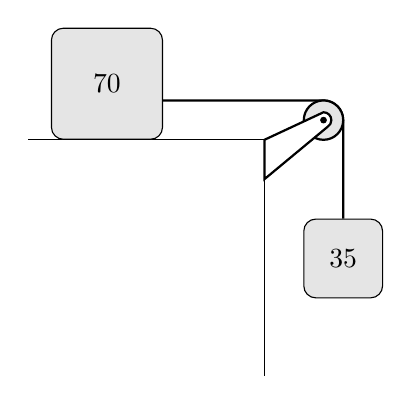
\begin{tikzpicture}
        %% Floor
        \draw (-3,0) -- (0,0) -- (0,-3);
        %% Mass
        \node[draw,fill=white!90!black,rectangle,rounded corners=1ex,minimum size=1.41cm,anchor=south] (A) at (-2,0) {\SI{70}{\newton}};
        \node[draw,fill=white!90!black,rectangle,rounded corners=1ex,minimum size=1.00cm,anchor=north] (B) at (1,-1) {\SI{35}{\newton}};
        %% Rope and Pulley
        \draw[thick] (A.south east) ++(90:0.5) -- (0.75,0.5) arc(90:0:0.25) -- (B.north);
        \draw[thick,fill=white!90!black] (0.75,0.25) circle (0.25); 
        \draw[thick,fill=white] (0,0) -- (0.75,0.35) arc (90:-60:0.1) -- (0,-0.5) -- cycle;
        \draw[fill] (0.75,0.25) circle (1pt);
        %% NOTE: Old
        %% Surface
        %\node[anchor=north,fill,pattern=north east lines,minimum width=3cm, minimum height=0.05cm] at (-1.5,0) {};
        %\node[anchor=east,fill,pattern=north east lines,minimum width=0.05cm, minimum height=2cm] at (0,-1) {};
        %\draw (-3,0) -- (0,0) -- (0,-2);
        %% Masses
        %\node[draw,fill=white!90!black,rectangle,minimum size=1.41cm,anchor=south] (A) at (-2,0) {\SI{70}{\newton}};
        %\node[draw,fill=white!90!black,rectangle,minimum size=1.00cm,anchor=north] (B) at (+0.75,-2) {\SI{35}{\newton}};
        %% Rope
        %\draw[thick] (A.south east) ++(90:0.5) -- (0.5,0.5) arc(90:0:0.25) -- (B.north);
        %% Pulley
        %\draw[fill=white!90!black] (0.5,0.25) circle (0.25);
        %\draw[fill] (0.5,0.25) circle (1.5pt);
        %\draw[fill] (0,0) circle (1.5pt);
        %\draw[fill] (0,-0.5) circle (1.5pt);
        %\draw[thick] (0,0) -- (0.5,0.25);
        %\draw[thick] (0,-0.5) -- (0.5,0.25);
    \end{tikzpicture}
    \end{center}
    If the pulley is massless and the surface is frictionless,
        the magnitude of the acceleration of the \SI{35}{\newton} block is:
    \begin{multicols}{3}
    \begin{choices}
        \wrongchoice{\SI{1.6}{\meter\per\second\squared}}
      \correctchoice{\SI{3.3}{\meter\per\second\squared}}
        \wrongchoice{\SI{4.9}{\meter\per\second\squared}}
        \wrongchoice{\SI{6.7}{\meter\per\second\squared}}
        \wrongchoice{\SI{9.8}{\meter\per\second\squared}}
    \end{choices}
    \end{multicols}
\end{question}
}

\element{halliday-mc}{
\begin{question}{halliday-ch05-q61}
    A \SI{13}{\newton} weight and a \SI{12}{\newton} weight are connected by a massless string over a massless,
        frictionless pulley.
    The \SI{13}{\newton} weight has a downward acceleration with magnitude equal to that of a freely falling body times:
    \begin{multicols}{3}
    \begin{choices}
        \wrongchoice{$1$}
        \wrongchoice{$\dfrac{1}{12}$}
        \wrongchoice{$\dfrac{1}{13}$}
      \correctchoice{$\dfrac{1}{25}$}
        \wrongchoice{$\dfrac{13}{25}$}
    \end{choices}
    \end{multicols}
\end{question}
}

\element{halliday-mc}{
\begin{question}{halliday-ch05-q62}
    A massless rope passes over a massless pulley suspended from the ceiling.
    A \SI{4}{\kilo\gram} block is attached to one end and a \SI{5}{\kilo\gram} block is attached to the other end.
    The acceleration of the \SI{5}{\kilo\gram} block is:
    \begin{multicols}{3}
    \begin{choices}
        \wrongchoice{$\dfrac{g}{4}$}
        \wrongchoice{$\dfrac{5g}{9}$}
        \wrongchoice{$\dfrac{4g}{9}$}
        \wrongchoice{$\dfrac{g}{5}$}
      \correctchoice{$\dfrac{g}{9}$}
    \end{choices}
    \end{multicols}
\end{question}
}

\element{halliday-mc}{
\begin{question}{halliday-ch05-q63}
    Two blocks, weighing \SI{250}{\newton} and \SI{350}{\newton},
        respectively, are connected by a string that passes over a massless pulley as shown.
    \begin{center}
    \begin{tikzpicture}
        %% Ceiling
        \node[anchor=south,fill,pattern=north east lines,minimum width=3cm, minimum height=0.05cm] at (0,0) {};
        \draw (-1.5,0) -- (1.5,0);
        %% Masses
        \node[draw,fill=white!90!black,rectangle,rounded corners=1ex,minimum size=1.00cm] (A) at (-0.75,-3) {\SI{250}{\newton}};
        \node[draw,fill=white!90!black,rectangle,rounded corners=1ex,minimum size=1.22cm] (B) at (+0.75,-4) {\SI{350}{\newton}};
        %% Rope
        \draw[thick] (A.north) -- (-0.75,-1) arc(180:0:0.75) -- (B.north);
        %% Pulley
        \draw[thick] (0,-1.00) circle (0.75);
        \draw[fill=white!50!black] (-0.25,0) -- (-0.15,-1.1) arc(190:350:0.15) -- (0.25,0) --cycle;
        \draw[fill] (0,-1.00) circle (1.5pt);
        %% NOTE: Old
        %% Ceiling
        %\node[anchor=south,fill,pattern=north east lines,minimum width=2cm, minimum height=0.05cm] at (0,0) {};
        %\draw (-1,0) -- (1,0);
        %% Masses
        %\node[draw,fill=white!90!black,rectangle,minimum size=1.18cm] (A) at (0.75,-4) {\SI{350}{\newton}};
        %\node[draw,fill=white!90!black,rectangle,minimum size=1.00cm] (B) at (-0.75,-3) {\SI{250}{\newton}};
        %% Rope
        %\draw[thick] (A.north) -- (0.75,-1.00) arc(0:180:0.75) -- (B.north);
        %% Pulley
        %\draw[fill=white!90!black] (0,-1) circle (0.75);
        %\draw[fill] (0,0) circle (1.5pt);
        %\draw[fill] (0,-1) circle (1.5pt);
        %\draw[thick] (0,0) -- (0,-1);
    \end{tikzpicture}
    \end{center}
    The tension in the string is:
    \begin{multicols}{3}
    \begin{choices}
        \wrongchoice{\SI{210}{\newton}}
      \correctchoice{\SI{290}{\newton}}
        \wrongchoice{\SI{410}{\newton}}
        \wrongchoice{\SI{500}{\newton}}
        \wrongchoice{\SI{4900}{\newton}}
    \end{choices}
    \end{multicols}
\end{question}
}

\newcommand{\hallidayChFiveQSixtyFour}{
\begin{tikzpicture}
    %% Table
    \node[fill,pattern=north east lines,anchor=north,minimum width=4cm,minimum height=0.50cm] at (0,0) {};
    \draw (-2,-0.50) rectangle (+2,0);
    \draw[fill] (-1.9,-0.5) rectangle (-1.95,-1.00);
    \draw[fill] (+1.9,-0.5) rectangle (+1.95,-1.00);
    %% Masses
    \node[draw,fill=white!90!black,rectangle,anchor=south,minimum height=0.50cm,minimum width=3cm] (A) at (0,0) {\SI{10}{\newton}};
    \node[draw,fill=white!90!black,rectangle,anchor=south,minimum height=0.50cm,minimum width=2.5cm] (B) at (A.north) {\SI{5}{\newton}};
    \node[draw,fill=white!90!black,rectangle,anchor=south,minimum height=0.50cm,minimum width=2.0cm] (C) at (B.north) {\SI{4}{\newton}};
    %% Labels
    \node[anchor=east] at (A.west) {$Z$};
    \node[anchor=east] at (B.west) {$Y$};
    \node[anchor=east] at (C.west) {$X$};
\end{tikzpicture}
}

\element{halliday-mc}{
\begin{question}{halliday-ch05-q64}
    Three books ($X$, $Y$, and $Z$) rest on a table.
    \begin{center}
        \hallidayChFiveQSixtyFour
    \end{center}
    The weight of each book is indicated.
    The net force acting on book $Y$ is:
    \begin{multicols}{2}
    \begin{choices}
        \wrongchoice{\SI{4}{\newton} down}
        \wrongchoice{\SI{5}{\newton} up}
        \wrongchoice{\SI{9}{\newton} down}
      \correctchoice{zero}
        \wrongchoice{none of these}
    \end{choices}
    \end{multicols}
\end{question}
}

\element{halliday-mc}{
\begin{question}{halliday-ch05-q65}
    Three books ($X$, $Y$, and $Z$) rest on a table.
    \begin{center}
        \hallidayChFiveQSixtyFour
    \end{center}
    The weight of each book is indicated.
    The force of book $Z$ on book $Y$ is:
    \begin{multicols}{3}
    \begin{choices}
        \wrongchoice{zero}
        \wrongchoice{\SI{5}{\newton}}
      \correctchoice{\SI{9}{\newton}}
        \wrongchoice{\SI{14}{\newton}}
        \wrongchoice{\SI{19}{\newton}}
    \end{choices}
    \end{multicols}
\end{question}
}

\element{halliday-mc}{
\begin{question}{halliday-ch05-q66}
    Three blocks ($A$, $B$, $C$), each having mass $M$,
        are connected by strings as shown.
    \begin{center}
    \begin{tikzpicture}
        %% Surface
        \node[fill,pattern=north east lines,anchor=north,minimum width=6cm,minimum height=0.05cm] at (0,0) {};
        \draw (-3,0) -- (+3,0);
        %% blocks
        \node[draw,fill=white!90!black,rectangle,minimum size=1.00cm,anchor=south] (A) at (-1.5,0) {$A$};
        \node[draw,fill=white!90!black,rectangle,minimum size=1.00cm,anchor=south] (B) at (+0.0,0) {$B$};
        \node[draw,fill=white!90!black,rectangle,minimum size=1.00cm,anchor=south] (C) at (+1.5,0) {$C$};
        %% String
        \draw[thick] (A.east) -- (B.west);
        \draw[thick] (B.east) -- (C.west);
        \draw[thick,->] (C.east) -- ++(0:1) node[pos=0.5,anchor=south] {$F$};
    \end{tikzpicture}
    \end{center}
    Block $C$ is pulled to the right by a force $F$ that causes the entire system to accelerate.
    Neglecting friction, the net force acting on block $B$ is:
    \begin{multicols}{3}
    \begin{choices}
        \wrongchoice{zero}
      \correctchoice{$\dfrac{F}{3}$}
        \wrongchoice{$\dfrac{F}{2}$}
        \wrongchoice{$\dfrac{2 F}{3}$}
        \wrongchoice{$F$}
    \end{choices}
    \end{multicols}
\end{question}
}

\element{halliday-mc}{
\begin{question}{halliday-ch05-q67}
    Two blocks with masses $m$ and $M$ are pushed along a horizontal
        frictionless surface by a horizontal applied force $F$ as shown.
    \begin{center}
    \begin{tikzpicture}
        %% Surface
        \node[fill,pattern=north east lines,anchor=north,minimum width=4cm,minimum height=0.05cm] at (0,0) {};
        \draw (-2,0) -- (+2,0);
        %% blocks
        \node[draw,fill=white!90!black,rectangle,minimum size=1.42cm,anchor=south east] (A) at (0,0) {$M$};
        \node[draw,fill=white!90!black,rectangle,minimum size=1.00cm,anchor=south west] (B) at (0,0) {$m$};
        %% String
        \draw[thick,<-] (A.west) -- ++(180:2) node[pos=0.5,anchor=south] {$F$};
    \end{tikzpicture}
    \end{center}
    The magnitude of the force of either of these blocks on the other is:
    \begin{multicols}{3}
    \begin{choices}
      \correctchoice{$\dfrac{m F}{m + M}$}
        \wrongchoice{$\dfrac{m F}{M}$}
        \wrongchoice{$\dfrac{m F}{M - m}$}
        \wrongchoice{$\dfrac{M F}{M + m}$}
        \wrongchoice{$\dfrac{M F}{m}$}
    \end{choices}
    \end{multicols}
\end{question}
}

\element{halliday-mc}{
\begin{question}{halliday-ch05-q68}
    Two blocks ($A$ and $B$) are in contact on a horizontal frictionless surface.
    A \SI{36}{\newton} constant force is applied to $A$ as shown.
    \begin{center}
    \begin{tikzpicture}
        %% Surface
        \node[fill,pattern=north east lines,anchor=north,minimum width=4cm,minimum height=0.05cm] at (0,0) {};
        \draw (-2,0) -- (+2,0);
        %% blocks
        \node[draw,fill=white!90!black,rectangle,minimum size=1.00cm,anchor=south east] (A) at (0,0) {$A$};
        \node[draw,fill=white!90!black,rectangle,minimum size=1.42cm,anchor=south west] (B) at (0,0) {$B$};
        %% String
        \draw[thick,<-] (A.west) -- ++(180:2) node[pos=0.5,anchor=south] {\SI{36}{\newton}};
    \end{tikzpicture}
    \end{center}
    If $m_A=\SI{4.0}{\kilo\gram}$, and $m_B=\SI{20}{\kilo\gram}$,
        then the magnitude of the force of $A$ on $B$ is:
    \begin{multicols}{3}
    \begin{choices}
        \wrongchoice{\SI{1.5}{\newton}}
        \wrongchoice{\SI{6.0}{\newton}}
        \wrongchoice{\SI{29}{\newton}}
      \correctchoice{\SI{30}{\newton}}
        \wrongchoice{\SI{36}{\newton}}
    \end{choices}
    \end{multicols}
\end{question}
}

\element{halliday-mc}{
\begin{question}{halliday-ch05-q69}
    A short \SI{10}{\gram} string is used to pull a \SI{50}{\gram} toy across a frictionless horizontal surface.
    If a \SI{3.0e-2}{\newton} force is applied horizontally to the free end,
        the force of the string on the toy, at the other end, is:
    \begin{multicols}{2}
    \begin{choices}
        \wrongchoice{\SI{0.15}{\newton}}
        \wrongchoice{\SI{6.0e-3}{\newton}}
      \correctchoice{\SI{2.5e-2}{\newton}}
        \wrongchoice{\SI{3.0e-2}{\newton}}
        \wrongchoice{\SI{3.5e-2}{\newton}}
    \end{choices}
    \end{multicols}
\end{question}
}


\endinput


